%!TEX root = ../Bachelorarbeit.tex
\chapter{Motivation}
\label{chap:Einleitung}
Die School of Design Thinking (D-School) lehrt die kreative Herangehensweise an Probleme und die Entwicklung einfallsreicher Lösungen. Die Lehre findet dabei in verschiedenen Kursen statt. Studierende können sich die Grundlagen im \gls{Basic-Track} aneignen und nach erfolgreicher Teilnahme ihr Wissen im  \gls{Advanced-Track} vertiefen. Neben den studentischen Kursen bietet die D-School auch Weiterbildungskurse für Unternehmen an.

In der Regel besteht ein D-School Kurs aus mehreren Kleingruppen von ca. sechs Teilnehmern, die gemeinsam an einem Projekt arbeiten. Das Projektthema wird dabei entweder von der D-School selbst oder, vor allem bei längeren Projekten, von externen Projektpartnern vorgeschlagen. 

Bei der Arbeit an den Projekten durchlaufen die Teilnehmenden verschiedene Phasen: Während dabei zunächst das Verstehen und Beobachten des Problemfeldes im Vordergrund stehen, wird anschließend ein Standpunkt definiert. Es folgt die Phase der Ideenfindung, an die die Erstellung eines Prototypen anknüpft. Dieser Prototyp wird zum Schluss mit geeigneten Versuchspersonen getestet. Im Verlauf dieser Phasen entstehen unterschiedlichste Dokumente, welche die Lösungsfindung dokumentieren. (vgl. \cite{design-thinking})

Im Verlauf des Projektes kommt es durchaus vor, dass ein Team eine Phase mehrmals durchläuft oder in eine vorherige Phase zurückkehrt. Dies erschwert die Organisation der Dokumente, z.B. in einer einfachen hierarchischen Struktur. Weiterhin ist es schwierig allein aus den Dokumenten deren Entstehungsreihenfolge und Bedeutung zu erfassen. Meist entstehen während eines drei Monate andauernden Projektes verschiedenste Präsentationen, Zusammenfassungen, Prototypen, Bilder von Whiteboards und Interviewdokumentationen. Diese werden in der Regel in der von den Studierenden bevorzugten Art und Weise gespeichert und verwaltet, beispielsweise mit Hilfe von Dropbox\footnote{\url{http://www.dropbox.com}}, Google Docs\footnote{\url{http://drive.google.com}} oder \gls{Box}\footnote{\url{http://box.com}}.

Das Verständnis der Dokumentation ist sowohl für das Projekt selbst, zum Verstehen und Erlernen des Prozesses, als auch als Ideenquelle für zukünftige Projekte wichtig. Ferner sind die erstellten Artefakte nützlich um neue Projektpartner zum Werben, welche die Projekte betreuen. 

\section{Zielsetzung von Project-Zoom}
Project-Zoom soll der Verbesserung der Dokumentation dienen. Dazu sollen die von den Studierenden erzeugten Artefakte durch manuelles Anordnen in eine Form gebracht werden, welche den Prozess der Gruppe visualisiert. Die Mitarbeiter der D-School können diese entstandenen Graphen anschließend nutzen um die Projektverläufe zu analysieren und gegebenenfalls den D-School Prozess anpassen.

Für eine reibungslose Integration des Systems ist vor allem die Anbindung an bereits existierende IT-Systeme und die von den Studierenden für das Projekt verwendete Software wichtig. Ebendiese muss dabei mit moderatem Aufwand angepasst werden können, um andere externe Dienste anbinden zu können.

\section{Abgrenzung}
Die Arbeit beschreibt und bezieht sich auf das Bachelorprojekt „From Creative Ideas to Well-Founded Engineering“ und das umgesetzte Softwaresystem Project-Zoom. Insgesamt haben sechs Studierende an dem Projekt gearbeitet, die in ihren Bachelorarbeiten aus verschiedenen Blickwinkeln und mit verschiedenen Schwerpunkten Project-Zoom beschreiben.

Tom Herolds Arbeit \cite{bp-tomh} beinhaltet die Interaktion mit kontextsensitiven Graphen. Dabei geht es darum, den Umgang der Studierenden mit der Nutzeroberfläche so intuitiv wie möglich zu gestallten und den Nutzer bei der Erfassung dokumentationsrelevanter Eigenschaften zu unterstützen.

Die Ausführungen von Anita Diekhoff \cite{bp-anita}  beschäftigen sich mit der ...

Norman Rzepkas Bachelorarbeit \cite{bp-norman} thematisiert die webbasierte, eventgesteuerte, clientseitige Architektur von Project-Zoom. Hier wird näher darauf eingegangen, wie die Daten von der Datenbank, über das Backend asynchron an den Client ausgeliefert werden.

Die Bachelorarbeit von Dominic Bräunlein \cite{bp-dome} erläutert das Generieren und Bereitstellen von semantischen \gls{Thumbnails}, um dem Nutzer das Erkennen der Dokumente seines Projektes zu erleichtern und somit selbst bei wenig verfügbarem Platz so viele Informationen eines Dokumentes anzeigen zu können wie möglich. 

Thomas Werkmeister befasst sich in seiner Arbeit \cite{bp-tewe} mit der Anbindung externer Systeme zur Integration von Daten. Diese aggregierte Datenbasis ist die Grundlage für die Wissensbasis und die einzelnen Projekte.

\begin{figure}[h]  
  \centering     
  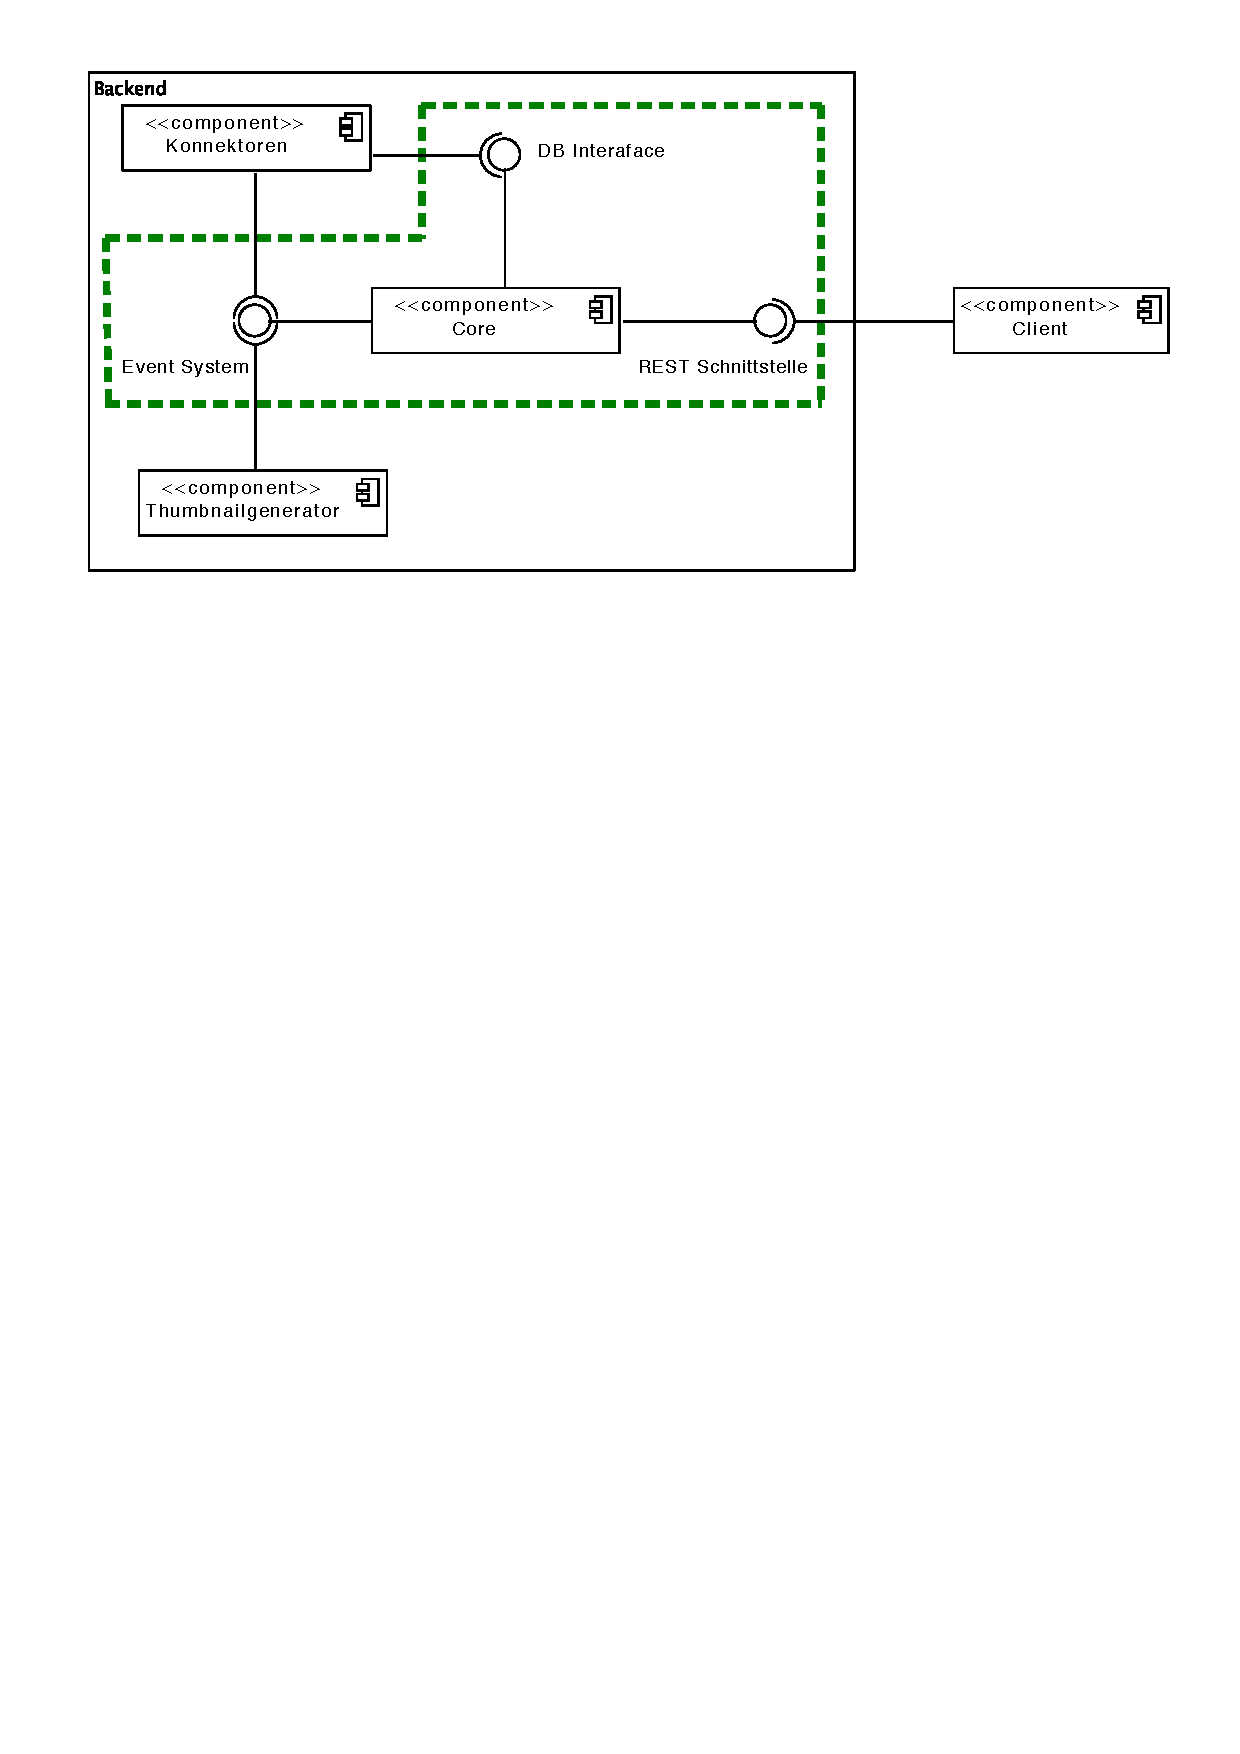
\includegraphics[width=1.0\textwidth]{img/architecture_overview.pdf}  
   \caption{Überblick über die verschiedenen Packete und ihre Schnittstellen; In gestricheltem Rahmen der für diese Arbeit relevante Teil der Architektur}
  \label{fig:architecture-overview} 
\end{figure}

Die Abbildung \ref{fig:architecture-overview} zeigt einen groben Überblick über die Architektur des Systems. Der für diese Arbeit relevante Teil ist dabei gestrichelt eingerahmt. Die Komponenten, die in den Arbeiten \cite{bp-tewe} (Konnektoren) und \cite{bp-dome} (Thumbnailgenerator) beschrieben sind, sind mit dem hier erläuterten Systemteil mittels eines Eventsystems verbunden. Das Client-Frontend ist über eine REST-Anbindung\footnote{vgl. Konzept des Representational state transfer in \cite{rest}} an das Server-Backend angeschlossen. Mit der clientseitigen Implementierung der REST-Schnittstelle beschäftigt sich \cite{bp-norman}.

In dieser Arbeit wird zunächst ein Überblick über das Gesamtsystem gegeben. Dazu werden die Anforderungen der D-School an das Backend analysiert, welche als Grundlage für die Wahl der verwendeten Technologien dienen. Anschließend wird die Architektur des Backends näher erläutert. Hier liegt der Hauptfokus zunächst auf einer neuen Art und Weise, eine Datenbank an eine Webapplikation anzubinden. Im Anschluss werden einige Feinheiten und ausgewählte Stellen der Datenmodellierung von Project-Zoom beleuchtet. Den Abschluss bildet die architekturelle Grundlage zur Anbindung externer Systeme für die Erweiterung von Project-Zoom.

%\zitat{"`Ein Zitat kann manchmal helfen ;-)"' (\cite{TODO})} 